\chapter{Diseño}
En un proyecto software, antes de comenzar a escribir código fuente, se debe realizar una
previa \textbf{elección de modelos en el diseño}, es decir, una elección de los distintos 
tipos/modelos de elementos que se quieren usar en la aplicación. Esta elección nos ayudará
en gran medida a la posterior elección de herramientas, explicada en el apartado
\ref{sec:tools}.\\

En los siguientes apartados, se explica y debaten las distintas posibilidades que habría en
la actualidad y por qué usar una u otra. Se desarrollarán los siguientes puntos:

    \begin{enumerate}
        \item Lenguaje nativo o framework web (\ref{sec:lenguaje-frameworkweb}).
        \item Patrones arquitectónicos de programación (\ref{sec:patrones-arquitectonicos}).
        \item Lenguaje CSS nativo o framework CSS (\ref{sec:css-frameworkcss}).
        \item Base de datos SQL o base de datos noSQL (\ref{sec:sql-nosql}).
    \end{enumerate}

\section{Lenguaje nativo o framework web} \label{sec:lenguaje-frameworkweb}
Antes de nada, vamos a explicar brevemente qué es un framework. Un \textbf{framework} es
un entorno o marco de trabajo que nos ofrece una estructura base con la que podemos
comenzar a elaborar un proyecto, es una especie de plantilla que es el punto de partida
para el comienzo y organización de un proyecto software. Éste permite agilizar mucho
el desarrollo, ya que se omiten tareas comunes o repetitivas.\\

Normalmente, cuando se tiene cierta experiencia programando, se van guardando códigos que
crees que pueden serte útiles en un futuro para ser \textbf{reutilizados}. Por ejemplo, un
sistema de login o de registro para una aplicación, ciertas funciones que verifican estados
concretos, etc. Dicho de forma coloquial, estos códigos que vamos creando y guardando son
nuestros \textbf{propios frameworks}. Este tipo de frameworks es lo que llamamos código
puro, o dicho metafóricamente, escribir código a pelo, código escrito directamente sin
ayuda de ninguna herramienta. Con esto en mente, ¿por qué debería usar un framework para
el desarrollo web? ¿por qué no podría usar mis propios frameworks simplemente? Pues bien,
las razones son sencillas:

    \begin{itemize}
        \item Tu código propio te puede servir a ti, pero...¿y a una \textbf{tercera persona}
        que tenga que trabajar en el mismo proyecto?
        \item Si en el proyecto participasen varios programadores y cada uno aportara
        funcionalidades de sus frameworks propios, sería muy difícil hacer que todo
        funcionase \textbf{conjuntamente}.
        \item Normalmente, si desarrollas tu propia aplicación sin frameworks, debes
        tener muchas más consideraciones acerca de la seguridad y probablemente puedas
        tener algún \textbf{agujero de seguridad} en tu código.
    \end{itemize}

Digamos que un framework web es un lugar de trabajo común donde muchos programadores
trabajan en conjunto. Esta es la principal razón por la que muchas empresas buscan
programadores que estén especializados con un framework determinado, para que se
\textit{"hablen el mismo idioma"} y puedan resolver tareas y dudas comunes.\\

Como aspectos negativos de usar un framework web hay muy pocos, aunque puede mencionarse
que normalmente suele haber modas en las que se usan determinados frameworks más que otros,
que pasan a caer en desuso.\\


\section{Patrones arquitectónicos de programación} \label{sec:patrones-arquitectonicos}
En la actualidad, existen multitud de patrones arquitectónicos para el desarrollo de
software, dichos patrones definen una forma concreta en la que los componentes principales
de una aplicación se comunican entre sí. Dado que nuestra aplicación tiene una parte de
desarrollo destinada al usuario (\textbf{UI, User Interface}), nos centraremos en el modelo
\textbf{Modelo-Vista-Controlador}.

\subsection{Modelo-Vista-Controlador} \label{sec:mvc}
Es el patrón más común entre los frameworks, éste se divide en tres bloques:

    \begin{itemize}
        \item \textbf{Modelo}: contiene toda la lógica relacionada con los datos.
        Interacciona de forma habitual con la base de datos mediante operaciones de
        \textbf{selección}, \textbf{inserción}, \textbf{actualización} y \textbf{eliminación}.
        Se comunica con el controlador.
        \item \textbf{Vista}: es la parte visible de la aplicación, es decir, la 
        \textbf{interfaz gráfica} visible al usuario y con la que éste interacciona.
        Normalmente está formada por código html, css y javascript, y se comunica con el
        controlador a través de las peticiones que el usuario realiza.
        \item \textbf{Controlador}: es el punto de unión entre el modelo y la vista. Éste
        procesa las \textbf{peticiones (requests)} que el usuario realiza a través de las
        vistas y las envía al modelo para que éste realice las operaciones necesarias y
        genere los datos correspondientes.
    \end{itemize}

El flujo de comunicación entre estos tres bloques es el siguiente:

    \begin{enumerate}
        \item El usuario (navegador) interacciona con la interfaz, generando una petición
        hacia el controlador.
        \item El controlador recibe la petición, la procesa, y la envía hacia el modelo
        si fuese necesario.
        \item Si el controlador ha mandado una petición al modelo, el modelo responde al
        controlador con la información solicitada. 
        \item El controlador manda la información hacia las vistas, que se actualizan con
        dicha información del modelo.
        \item Finalmente, el usuario puede ver las vistas con la información actualizada.
    \end{enumerate}

    \begin{figure}[H]
        \centering
        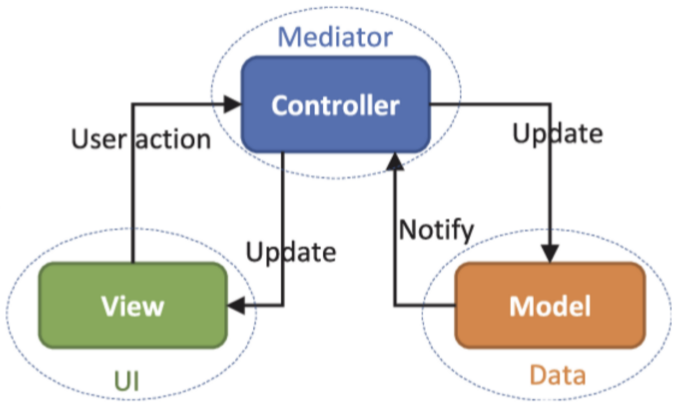
\includegraphics[scale=0.50]{imagenes/mvc.png}
        \caption[Patrón Modelo-Vista-Controlador]{Patrón Modelo-Vista-Controlador. Fuente \cite{mvc}}
        \label{fig:mvc}
    \end{figure}

Dado que vamos a utilizar un framework web para el desarrollo de la aplicación, y la gran
mayoría de ellos usan un modelo MVC, será el modelo que utilizaremos. Además, es el
patrón con el que más familiarizado estoy.

\section{Lenguaje CSS nativo o framework CSS} \label{sec:css-frameworkcss}
Hoy en día, suele haber soluciones software para casi todo, y el diseño para la interfaces
de usuario no iba a ser una excepción. Una de las principales razones para usar un framework
CSS es el \textbf{incremento de la productividad} durante el desarrollo de software, ya que,
al igual que los frameworks web, nos proporcionan gran cantidad de elementos ya definidos
como pueden ser componentes, estilos, formularios, etc. Entre las ventajas de usar un
framework CSS se encuentran:

    \begin{itemize}
        \item Acelera la realización de diseños y con ello la productividad.
        \item Posibilita el trabajo colaborativo, ya que todos los programadores
        trabajan en un mismo marco de trabajo.
        \item Permite generar un código más limpio y ordenado.
        \item Asegura la compatibilidad del código fuente entre navegadores.
    \end{itemize}

A pesar de tener muchas cosas buenas,también tiene algunas desventajas, entre las que
podemos mencionar las siguiente:

    \begin{itemize}
        \item Los principios de desacoplamiento entre código html y css se están perdiendo.
        \item En la maypría de ocasiones, el framework carga gran cantidad de código CSS
        que no se utilizará nunca.
        \item En ocasiones, el usarlo puede llevarte a desaprender conceptos de CSS que sí
        conocías anteriormente.
        \item Al ser frameworks usados por miles de usuarios, pueden encontrarse páginas
        muy similares a la desarrollada.
    \end{itemize}

Dado que en nuestra aplicación se tiene pensado hacer uso nativo de CSS, se van a
utilizar estos dos modelos: \textbf{CSS nativo} y un \textbf{framework CSS}.

\section{Base de datos SQL o base de datos noSQL} \label{sec:sql-nosql}
Antes de pasar a la elección de la Base de Datos concreta que vamos a utilizar, necesitamos
tener claro qué \textbf{tipo de base de datos} necesitamos, es decir, usar una base de datos
SQL o una base de datos noSQL. Comenzemos dando una breve definición de ambas:
    
    \begin{itemize}
        \item \textbf{Bases de Datos relacionales}: son aquellas que utilizan el lenguaje SQL
        (\textit{Structure Query Languaje}), un lenguaje de consulta estructurado. En este tipo
        de bases de datos los elementos se organizan en tablas. Cada fila hace referencia a un
        registro, es decir, a una instancia de esa tabla, mientras que las columnas representan
        campos de esos registros, teniendo un determinado tipo de dato cada una. En la
        actualidad, son el tipo de bases de datos más estándarizado y usado.
        \item \textbf{Base de Datos noSQL}: son aquellas bases de datos diseñadas para
        permitir grandes cantidades de datos, tipos de datos complejos, más índices,
        distintos tipos de consulta, etc. En este caso, no existen tablas donde se van
        almacenando los datos, sino que suelen utilizar un esquema clave-valor, documental,
        basado en grafos, etc. Este tipo de base de datos surgió para dar solución a los
        problemas de escalabilidad y rendimiento que las bases de datos relacionales
        generaban al haber miles de usuarios concurrentemente y realizando millones de
        consultas.
    \end{itemize}

En la siguiente tabla, se realiza una breve comparación entre ambos tipos: 

    \begin{table}[H]
        \begin{center}
            \begin{tabular}{ |l|l| } \hline
                \textbf{Base de datos SQL} & \textbf{Base de datos noSQL} \\ \hline
                SQL principal lenguaje & SQL como lenguaje de apoyo \\
                Tablas & Hashes, listas \\
                Permite operaciones JOIN & Problemas de rendimiento con JOIN \\
                Escalabilidad vertical & Escalabilidad horizontal \\
                Datos estructurados & Datos menos estructurados \\ 
                Arquitectura centralizada & Arquitectura distribuida \\
                Consistencia & Dinamicidad \\ \hline
            \end{tabular}
            \caption{tabla con la comparativa entre SQL y noSQL}
            \label{tab:databases}
        \end{center}
    \end{table}

Analizando la naturaleza de nuestro problema, observamos que existen elementos bien
distinguidos en una excavación, como son las \textbf{unidades estratigráficas}, los 
\textbf{hechos}, las \textbf{estancias}, los \textbf{materiales} que se encuentran formando
los hallazgos,....todo ello englobado dentro de las \textbf{excavaciones} y relacionados
unos con otros. Teniendo esto en cuenta, deberemos definir entidades y por tanto, es fácil
deducir que necesitaremos hacer uso de un sistema de almacenamiento que cumpla con el esquema
entidad-relación, es decir, de una \textbf{base de datos relacional o SQL}.
